\documentclass{uk_thesis}

% ~~~ PACKAGES ~~~
    \usepackage{diagbox} % for the corners of tables
    \usepackage{amsmath} % math and text, absolutely necessary!
    \usepackage{amsfonts} % for mathbb (used in number sets)
    \usepackage[dvipsnames]{xcolor} % colors and code command
    \usepackage{graphicx} % for includegraphics
    \usepackage{booktabs} % For formal tables
    \usepackage[ruled]{algorithm2e} % For algorithms
    \usepackage{yfonts} % To have basic fonts
    \usepackage{listings, scrhack} % For including of source code. scrhack removes warning produced by conflict in dependencies of listings and KOMA Script
    \usepackage{setspace} % For alternating between single and double spacing
    \usepackage{bookmark} % to add bookmarks to the PDF output, university requirement
    \usepackage{indentfirst} % indent every paragraph, including those after a section heading. Comment / uncomment this to toggle.
    \usepackage{csquotes} % With this package, use \enquote{text} to make smart quotes that use open and close quotes. These are context-sensitive and can be nested.
    \usepackage{amsthm} % for "proof" environment
    \usepackage{natbib} % for citeauthor, citeyear

    % Filling generators: you should probably remove these!
    \usepackage{lipsum}
    \usepackage{blindtext}
% ~~~ END PACKAGES ~~~

% ~~~ DEFINITIONS ~~~

    % use \code{text} for Markdown-like inline code snippets.
    \newcommand{\code}[1]{\ttfamily{}#1\normalfont{}}

    \renewcommand{\cite}[1]{[\citeauthor{#1}, \citeyear{#1}]} % make cite an authoryear citation, special ones can be custom made.
    \newcommand{\citeyearonly}[1]{[\citeyear{#1}]}
    \newcommand{\citeauthoronly}[1]{[\citeauthor{#1}]}

    \newcommand{\R}{\mathbb{R}}
    \newcommand{\Z}{\mathbb{Z}}
    \newcommand{\C}{\mathbb{C}}
    \newcommand{\N}{\mathbb{N}}
    \newcommand{\xor}{\ifmmode{}\oplus{}\else{}\textit{exclusive OR}\fi}
    \newcommand{\rightshift}{\ensuremath\mathrm{ >> }}
    \newcommand{\tablepad}{\vspace{0.8cm}}

% ~~~ END DEFINITIONS ~~~

% ~~~ CONFIGURATIONS ~~~

    % Configuration for code listings: monospace, nice columns, line breaks with a marker
    \lstset{
    basicstyle=\ttfamily,
    columns=fullflexible,
    breaklines=true,
    postbreak=\mbox{{\(\hookrightarrow{}\)}\space},
    }

% ~~~ END CONFIGURATIONS ~~~


\begin{document}


\title{Your Super Fancy\\ Super Long Thesis Title}
\author{You Yourself You}
\dgs{Zongming Fei}
\director{Mirosław Truszczyński}{Computer Science}
\codirector{Richard Ehrenborg}{Mathematics}
\degree{Master of Science}
\orcid{https://orcid.org/0000-0001-2345-6789}
\college{Engineering}
\submissiondate{2021}{05}{05}
% \alignedcodirector{}
\abstract{
    \lipsum[1]
}
\keywords{algorithms, graph theory, cats, numerical analysis, computer algebra systems}
\dedication{To my lovely cat, Jeff.} % WARNING: see issue #3
\acknowledgements{
    \lipsum[1]
}

\frontmatter

\maketitle

\tableofcontents

% If you don't have tables, comment this out or remove it.
\listoftables

% If you don't have figures, comment this out or remove it.
\listoffigures

% list of additional files

\doublespacing{}
\mainmatter{}
% Example thesis body. All of the mainmatter chapters.
% Of course you can also input other TeX files as well.

\chapter{Example thesis body}

  \section{Figures}

    LaTeX's neat, but it can be frustrating sometimes. Here is an example figure to help keep you from running into reference / spacing issues. Order matters!

    \begin{figure}
      \centering
      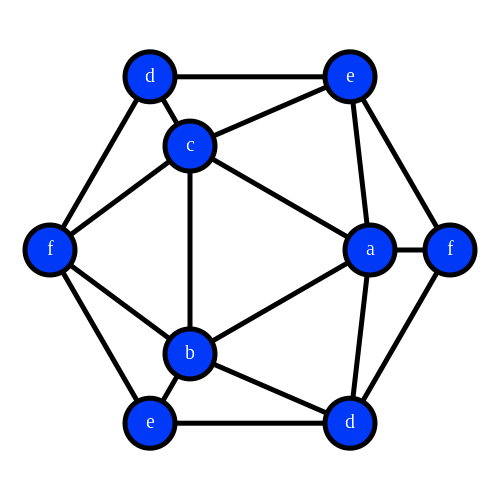
\includegraphics[scale=0.35]{res/images/pretty_picture.png}
      \caption{A beautiful depiction of something.}
      \label{fig:pretty_picture}
    \end{figure}

    See Figure \ref{fig:pretty_picture} for a pretty picture. Isn't it lovely? By the way, it is much easier to include PNGs than SVGs in LaTeX. 

    \lipsum{17}

  \section{Tables}

    LaTeX's neat, but it can be frustrating sometimes. See Table \ref{table:cool_table} for an example table to help keep you from running into reference / spacing issues. University requirements say that the caption should be above the table, which is why it is the way it is.

      \begin{table}
        \centering
        \caption{What a cool table}
        \label{table:cool_table}
        \tablecaptionpadding{}
        \begin{tabular}{c|cc}
          \diagbox{$a$}{$b$} & 0 & 1 \\\hline
          0 & 0 & 0 \\
          1 & 1 & 0 \\
        \end{tabular}
      \end{table}


    \lipsum{17}
  
  \section{References}

    I like to do my references this way, but it is not a hard requirement. I used the \code{natbib} package to create granular author / year citations with \code{hyperref} support.

    Examples:
    \begin{itemize}
      \item Author and year: \cite{vella:cat_breeding}
      \item Author only: \citeauthoronly{vella:cat_breeding}
      \item Year only: \citeyearonly{vella:cat_breeding}
    \end{itemize}

\blinddocument

\singlespacing{}


\appendix
\backmatter{}

\chapter{Appendices}

    \small

    % chapter* 's are quite unhelpfully not added to the table of contents.
    % must add manually
    \addcontentsline{toc}{section}{Results of tests}
    \section*{Results of tests}\label{chapter:results_of_tests}

    \addcontentsline{toc}{section}{Source code}
    \section*{Source code}

        \lstinputlisting[language=C++]{res/code_snippets/main.cpp}

    \normalfont{}


\bibliographystyle{apalike}
\bibliography{bibliography}

\pagebreak

\chapter{Vita}

    \begin{center}You Yourself You\end{center}

    \section*{Education}

      \begin{itemize}
        \item B.S. in Mathematics from the University of Kentucky. May, 2021.
        \item B.S. in Computer Science from the University of Kentucky. Expected May, 2022.
      \end{itemize}


    \section*{Professional positions held}

        \begin{itemize}
            \item Summer 2018 and Summer 2019: Cat Herding Apprentice at the Cat Reservation.
            \item September 2018 to January 2020: Cat Fur Trimmer at the Pet Store.
            \item September 2019 to October 2020: Professional Cat Petter at the Society of Cat Petting.
        \end{itemize}

    \section*{Scholastic and professional honors}

        \begin{itemize}
            \item Recognized as a Super Scholastic Human Being at the University of Kentucky: Fall 2019.
            \item Dean's List: Forever.
        \end{itemize}

\end{document}
